\documentclass[11pt,twoside,lineno]{pnas-new} % was: twocolumn

% Add supporting info as file dependency so that we can reference the figures
\makeatletter
\newcommand*{\addFileDependency}[1]{% argument=file name and extension
  \typeout{(#1)}
  \@addtofilelist{#1}
  \IfFileExists{#1}{}{\typeout{No file #1.}}
}

\usepackage[backend=bibtex,style=nature]{biblatex} % Borrowing citation formatting from Nature, also not necessarily going there

\usepackage{xr}
\addFileDependency{manuscript/text_supporting.tex}%
\addFileDependency{manuscript/text_supporting.aux}%
\externaldocument{manuscript/text_supporting}%

\usepackage{setspace} % double-spacing

\bibliography{references}

\newcommand\focalcountry{CHE}
\newcommand\mindate{01. Jan. 2020}
\newcommand\maxdate{01. Dec. 2020}
\newcommand\maxmissing{2903}
\newcommand\minlength{27000}
\newcommand\maxsamplingfraction{0.05}
\newcommand\subsamplebycanton{TRUE}
\newcommand\travelcontextscalefactor{0}
\newcommand\similaritycontextscalefactor{2}
\newcommand\traveldataweights{1,1,1}
\newcommand\whichtrees{\.*}
\newcommand\pickchainsunderothercriteria{TRUE}
\newcommand\ntrees{-1}
\newcommand\smoothconfcases{FALSE}
\newcommand\outgroupgisaidepiisls{EPI\_ISL\_406798}
\newcommand\uniquecontextonly{FALSE}
\newcommand\maskfromstart{100}
\newcommand\maskfromend{50}

\newcommand\nchainsmin{746}
\newcommand\nchainsmax{2995}
\newcommand\minlargestchainsper{23}
\newcommand\maxlargestchainsper{14}
\newcommand\nspanningchainsmin{}
\newcommand\nspanningchainsmax{}

\newcommand\nfocalsamples{5520}
\newcommand\nsimcontext{11009}
\newcommand\ntravelcontext{0}
\newcommand\meanweeklysamplingpercent{NaN}
\newcommand\minweeklysamplingpercent{NaN}
\newcommand\maxweeklysamplingpercent{NaN}
\newcommand\overallsamplingpercent{1.4}

\newcommand\summer_max_dampling_percent_median_CHE_no_sampUB{37}
\newcommand\summer_min_dampling_percent_median_CHE_no_sampUB{65}

\newcommand\medpersistenceatlockdownmin{27.5}
\newcommand\medpersistenceatlockdownmax{0}
\newcommand\qonepersistenceatlockdownmin{5.75}
\newcommand\qonepersistenceatlockdownmax{0}
\newcommand\qthreepersistenceatlockdownmin{58.5}
\newcommand\qthreepersistenceatlockdownmax{1}
\newcommand\medpersistenceatpeakmin{174}
\newcommand\medpersistenceatpeakmax{167}
\newcommand\qonepersistenceatpeakmin{163}
\newcommand\qonepersistenceatpeakmax{111}
\newcommand\qthreepersistenceatpeakmin{192}
\newcommand\qthreepersistenceatpeakmax{169.5}

\newcommand\casescoeffmax{0.048}
\newcommand\casescoeffmin{0.0074}
\newcommand\casesdelaymax{2}
\newcommand\casesdelaymin{5}
\newcommand\introsavertedmax{4038}
\newcommand\introsavertedmin{593}
\newcommand\introsavertedaspermax{84}
\newcommand\introsavertedaspermin{83}


\templatetype{pnasresearcharticle} % Borrowing template from PNAS, not necessarily going there 1st

\title{Genomic data enable quantification of the effect of  public health measures on reducing introductions and slowing local transmission in the 2020 Swiss SARS-CoV-2 epidemic}

% Use letters for affiliations, numbers to indicate the corresponding author
\author[a,b]{Sarah A. Nadeau}
\author[a,b]{Timothy G. Vaughan} 
\author[c]{Christiane Beckmann}
\author[a,b]{Ivan Topolsky}
\author[a,b]{Chaoran Chen}
\author[b,d]{Emma Hodcroft}
\author[a]{Tobias Schär}
\author[a]{Ina Nissen}
\author[a]{Natascha Santacroce}
\author[a]{Elodie Burcklen}
\author[a,b]{Pedro Ferreira}
\author[a,b]{Kim Philipp Jablonski}
\author[a,b]{Susana Posada-Céspedes}
\author[a]{Vincenzo Capece}
\author[a,b]{Sophie Seidel}
\author[e]{Noemi Santamaria de Souza}
\author[f]{Julia M. Martinez-Gomez}
\author[f]{Phil Cheng}
\author[f]{Philipp P. Bosshard}
\author[f]{Mitchell P. Levesque}
\author[g]{Verena Kufner}
\author[g]{Stefan Schmutz}
\author[g]{Maryam Zaheri}
\author[g]{Michael Huber}
\author[g]{Alexandra Trkola}
\author[h]{Samuel Cordey}
\author[h]{Florian Laubscher}
\author[i]{Ana Rita Gonçalves}
\author[j]{Sébastien Aeby}
\author[j]{Trestan Pillonel}
\author[j]{Damien Jacot}
\author[j]{Claire Bertelli}
\author[j]{Gilbert Greub}
\author[k,l]{Karoline Leuzinger}
\author[m,b,n]{Madlen Stange}
\author[m,b,n]{Alfredo Mari}
\author[m,b]{Tim Roloff}
\author[m,b]{Helena Seth-Smith}
\author[n]{Hans H. Hirsch}
\author[m,n]{Adrian Egli}
\author[c]{Maurice Redondo}
\author[c]{Olivier Kobel}
\author[c]{Christoph Noppen}
\author[a,b]{Niko Beerenwinkel}
\author[b,o]{Richard A. Neher}
\author[a]{Christian Beisel}
\author[a,b,1]{Tanja Stadler}

\affil[a]{Department of Biosystems Science and Engineering, ETH Zürich, Basel, Switzerland}
\affil[b]{Swiss Institute of Bioinformatics, Lausanne, Switzerland}
\affil[c]{Viollier AG, Allschwil, Switzerland}
\affil[d]{Institute for Social and Preventive Medicine, University of Bern, Bern, Switzerland}
\affil[e]{Department of Biology, ETH Zürich, Zürich, Switzerland}
\affil[f]{Department of Dermatology, University Hospital Zurich, University of Zürich, Zürich, Switzerland}
\affil[g]{Institute of Medical Virology, University of Zürich, Zürich, Switzerland}
\affil[h]{Laboratory of Virology, Division of Infectious Diseases and Division of Laboratory Medicine, University Hospitals of Geneva \& Faculty of Medicine, University of Geneva, Geneva, Switzerland}
\affil[i]{Swiss National Reference Centre for Influenza, University Hospitals of Geneva, Geneva, Switzerland}
\affil[j]{Institute of Microbiology, University Hospital Centre and University of Lausanne, Lausanne, Switzerland}
\affil[k]{Clinical Virology, University Hospital Basel, Basel, Switzerland}
\affil[l]{Transplantation \& Clinical Virology, Department Biomedicine, University of Basel, Basel, Switzerland}
\affil[m]{Clinical Bacteriology and Mycology, University Hospital Basel, Basel, Switzerland}
\affil[n]{Applied Microbiology Research, Department of Biomedicine, University of Basel, Basel, Switzerland}
\affil[o]{Biozentrum, University of Basel, Basel, Switzerland}

% Please include corresponding author, author contribution and author declaration information
% \authorcontributions{Please provide details of author contributions here.}
% \authordeclaration{Please declare any competing interests here.}
\correspondingauthor{\textsuperscript{1}To whom correspondence should be addressed. E-mail: tanja.stadler@bsse.ethz.ch}

% Three to five keywords, separated by the pipe symbol.
\keywords{Epidemiology $|$ SARS-CoV-2 $|$ Phylogenetics $|$ Phylodynamics} 

\begin{abstract}
% Please provide an abstract of no more than 250 words in a single paragraph. Abstracts should explain to the general reader the major contributions of the article. References in the abstract must be cited in full within the abstract itself and cited in the text.
Pathogen genome sequences are a unique source of information to trace routes of infection and track transmission dynamics through time. We sequenced 11,357 SARS-CoV-2 genomes in Switzerland throughout 2020 - the 6th largest sequencing effort during this period globally. Here we used this large data set to quantify introduction and transmission dynamics in Switzerland from a representative subset of all Swiss sequences from 2020. First, we identified putatively independent introductions of SARS-CoV-2 and tracked their persistence using phylogenetic methods. By comparing our genome-based estimates to expected values under simple null models without intervention measures, we can report that reduced travel around Switzerland's spring border closures averted \introsavertedmin\ - \introsavertedmax\ introductions, a reduction of approximately 83\%. We estimate that introductions circulating at the start of Switzerland's partial lockdown persisted around half as long as at a post-lockdown peak, though genome-based signal is much noisier here. Finally, we implemented a novel phylodynamic model to test for evidence of successful contact tracing, reasoning that contact tracing can only slow newly introduced outbreaks once they are detected. Using this model, we confirm the reproductive number of SARS-CoV-2 dropped from XX to XX coinciding with the partial lockdown start. We additionally report that across summer 2020 introductions, transmission in newly introduced outbreaks slowed \summermaxdampingpercentmedianCHEnosampUB\ - \summermindampingpercentmedianCHEnosampUB\% at the time of genome sampling. A plausible explanation of this summertime ``slowdown'' dynamic is a successful test-trace-isolate implementation that roughly halved transmissions once an introduction was identified. This slowdown is not detected in fall which might point to contact tracing having been overburdened during the fall wave. Our analysis based on genomic sequencing data helps quantify the effects of international travel, general measures, and specific contact tracing efforts towards a national epidemic, an increasingly relevant topic as global vaccination campaigns continue at an uneven pace and new variants of concern spread internationally.
\end{abstract}



\begin{document}

\maketitle
\abscontentformatted
\doublespacing

\section{Introduction}

% Claim importance
A crucial task in public health is to evaluate measures aimed at slowing SARS-CoV-2 transmission. Such measures aim to prevent new introductions into a region or contain ongoing transmission chains, for example with quarantine for travellers or social distancing. So far, mathematical models have helped estimate effects from broad measures like travel bans and lockdowns. These methods use data on case or death counts and travel volumes, e.g. \cite{Flaxman2020, Tian2020}. However, these data are not informative at the scale of individual introductions or transmission chains because there is no information to link related cases.

Detailed contact tracing data could help link cases to reconstruct introductions and transmission chains. However, these data are difficult to collect and not widely available. Instead, pathogen genome sequences can be used to link cases \cite{Kraemer}. Many RNA viruses accumulate mutations on the same time-scale as host-to-host transmission. For example a typical SARS-CoV-2 strain will accumulate $\sim$2 mutations per month along its $\sim$30,000 nucleotide-long genome \cite{Nextstrainteam}. These mutations allow us to construct a viral phylogeny (a ``family tree'' of viruses) that approximates the underlying host-to-host transmission tree. Where contact tracing data is available, this approach has been verified and has even helped link unassigned individuals to known transmission chains \cite{Rockett2020, Mendes2021}.

SARS-CoV-2 genomes were collected at an unprecedented scale in 2020 \cite{Alm2020} and they have been extensively used to characterize transmission dynamics. Two broad categories of methods are commonly employed: phylogenetic and phylodynamic methods. Phylogenetic studies reconstruct a ``best-guess'' phylogeny and calculate statistics directly from this phylogeny without further explicit models. For example, \cite{Mallon2020, DuPlessis2021} showed that national lock-downs during the early Irish and English epidemics reduced lineage sizes and diversity according to reconstructed phylogenies. Phylodynamic studies assume the phylogeny must arise from some underlying model of transmission between hosts (and possibly migration of hosts between regions). This approach enables estimation of population-level transmission dynamics. For example, \cite{Miller2020, Geoghegan2020a, muller-wa-covid} showed that public health measures reduced SARS-CoV-2 transmission rates in Israel, New Zealand, and Washington State, USA. 

% Indicate a gap
It is rather difficult to quantify effects of public health measures using genomic data. Firstly, sequencing efforts vary by region and through time. Often, available samples are unrepresentative of the entire population \cite{Villabona-Arenas2020, DeMaio2015}. Secondly, SARS-CoV-2 sequencing was high compared to viral diversity, in particular during the early epidemic in spring 2020 \cite{Morel2021}. If many sequences are similar or identical, the phylogeny will contain polytomies. This means the phylogeny is only a coarse approximation of the  host-to-host transmission tree \cite{Villabona-Arenas2020}. Even worse, arbitrarily resolving polytomies may give misleading or overly confident estimates \cite{Morel2021}. Finally, real-world transmission dynamics are governed by complex population structure that is difficult to model. Highly parameterized phylodynamic models can help, as in \cite{Miller2020, Geoghegan2020a, Muller2020a}. Models with multiple compartments account for sampling biases and population structure and the phylogeny can be integrated out as a nuisance parameter. Recent developments are speeding these methods up \cite{Lemey2021}, but they are generally too computationally complex to fit to thousands of genomes.

% State that our paper fills the gap 
Here we developed a two-step analysis framework carefully combining phylogenetic and phylodynamic methods to address these challenges and quantify transmission dynamics throughout 2020 in Switzerland. In each step, we condition on partitions of the full sample set, an approach inspired by  \cite{Muller2020} and \cite{DuPlessis2021}. First we restrict our search for introductions into Switzerland to within each Pango lineage \cite{Rambaut2000}, aggregating Swiss lineages into their parent lineages to ensure each lineage originates abroad. Then, we condition our phylodynamic inference on two extreme but plausible sets of identified introductions resulting from different polytomy resolutions. These procedures ensure computational feasibility. To limit sampling biases, we down-sample sequences to be more spatio-temporally representative of the Swiss epidemic. Finally, as mentioned, we account for phylogenetic uncertainty from high sampling and comparatively low viral diversity by conservatively reporting estimates across a range of extreme but plausible polytomy resolutions.

% Emphasize our aims 
We use our framework to quantify transmission dynamics in Switzerland, with a particular focus on the effects of public health measures on the Swiss epidemic. First, we asked when introductions occurred and how long they persisted in Switzerland. We compared genome-based estimates to expected values under simple null models without intervention measures to estimate the effect of the Swiss border closures and lockdown on these variables. We then asked how well introductions were controlled once they were identified by public health authorities. We reasoned that test-trace-isolate measures can only be enforced once authorities know about a case. Therefore, if successful, we hypothesized contact tracing efforts will slow transmission after the first case in a transmission chain is identified. We developed a novel phylodynamic model to test for this slowdown effect based on genome sequence data. Although we focused on the Swiss epidemic, our framework can be applied to any regional SARS-CoV-2 epidemic with data available on GISAID \cite{GISAID}. We performed a small comparison using New Zealand data to illustrate this. 

\section{Results}
We analyzed \nfocalsamples\ SARS-CoV-2 genomes collected in Switzerland, representing the Swiss epidemic from the first detected case on 25. Feb. through \maxdate. These data are a sub-sample of all available Swiss genomes aimed to be more spatio-temporally representative of the Swiss epidemic compared to all available genomes while maintaining a large sample size (Figure  \ref{fig:downsampling_representativeness}). We limited the sampling period to avoid transmission rate variation due to more transmissible variants of concern, such as alpha, which arose in late 2020.

\subsection{Introductions, then persistence characterize the 2020 Swiss epidemic}

First, we identified independent introductions of SARS-CoV-2 into Switzerland using genome data and estimated their persistence. To do this, we divided Swiss SARS-CoV-2 genome sequences into different Pango lineages (Table S1) and constructed an approximate maximum-likelihood phylogeny for each lineage of Swiss and genetically similar foreign sequences. Next, we identified independently introduced singleton sequences or clusters of Swiss sequences from these lineage phylogenies as described in the Methods. Importantly, we identified two different sets of introductions resulting from two extreme resolutions of polytomies in the phylogenies. This allows us to report estimates across the range of strictly bifurcating phylogenies consistent with the genome data. We refer to these different sets of plausible introductions as ``few'' or ``many'' introductions.

We estimate the analyzed sequences originate from between \nchainsmin\ (few) and \nchainsmax\ (many) independent introductions into Switzerland. These introductions are roughly power law-distributed in size, with the 10 largest introductions accounting for \maxlargestchainsper\ \% to \minlargestchainsper \% of genomes (Figure \ref{fig:chain_size_dist}). From a down-sampling analysis, we see that we do not reach saturation - if we were to include more sequences, we would identify more introductions (Figure \ref{fig:sensitivity_figs}a). Therefore, the true number of introductions into Switzerland is difficult to estimate using our phylogenetic approach. 

However, since we sampled genome sequences proportional to the number of confirmed cases through time, we expect that trends through time in the number and persistence of introductions are representative of the underlying dynamics. Figure \ref{fig:chain-longevity}A shows that the number of new introductions each week rose exponentially from Feb. to Mar. 2020, coinciding with an exponential rise in European cases during this time (Figure \ref{fig:chain-longevity}B). Newly sampled introductions into Switzerland peaked the week of 15. Mar. (Figure \ref{fig:chain-longevity}A). Switzerland closed its borders 13. Mar. 2020 \cite{SWI-border-closure}. Given the delay between the true date of introduction and sampling, introductions likely peaked well before cases in Switzerland's neighboring countries and the rest of Europe (Figure \ref{fig:chain-longevity}B). After the border closure, newly sampled introductions dropped week-on-week until the week of 14. Jun. Switzerland re-opened its borders 15. Jun. 2020. Then, newly sampled introductions rose more-or-less steadily until Nov. 2020, coinciding with borders reopening across Europe and globally. 

Of course, new introductions cannot sustain a local epidemic unless they persist in the local population. Our analysis suggests several introductions were quite persistent in Switzerland, including \nspanningchainsfebnovmin\ that may have persisted from the start of the Swiss epidemic in Feb. 2020 until Nov. 2020 (Figure \ref{fig:chain-longevity-matrix}). On average, introductions persisted in Switzerland \meantimetolastsamplemax\ - \meantimetolastsamplemin\ days from first to last sampling. However, introductions in early 2020 were less persistent than later introductions. Figure \ref{fig:chain-longevity} shows the fraction of newly sampled introductions each month that persist at least 60 days. 0.5 - 8\% of Apr. introductions persisted this long, compared to 12 - 52\% of Sep. introductions. 

\begin{figure}[H]
\centering
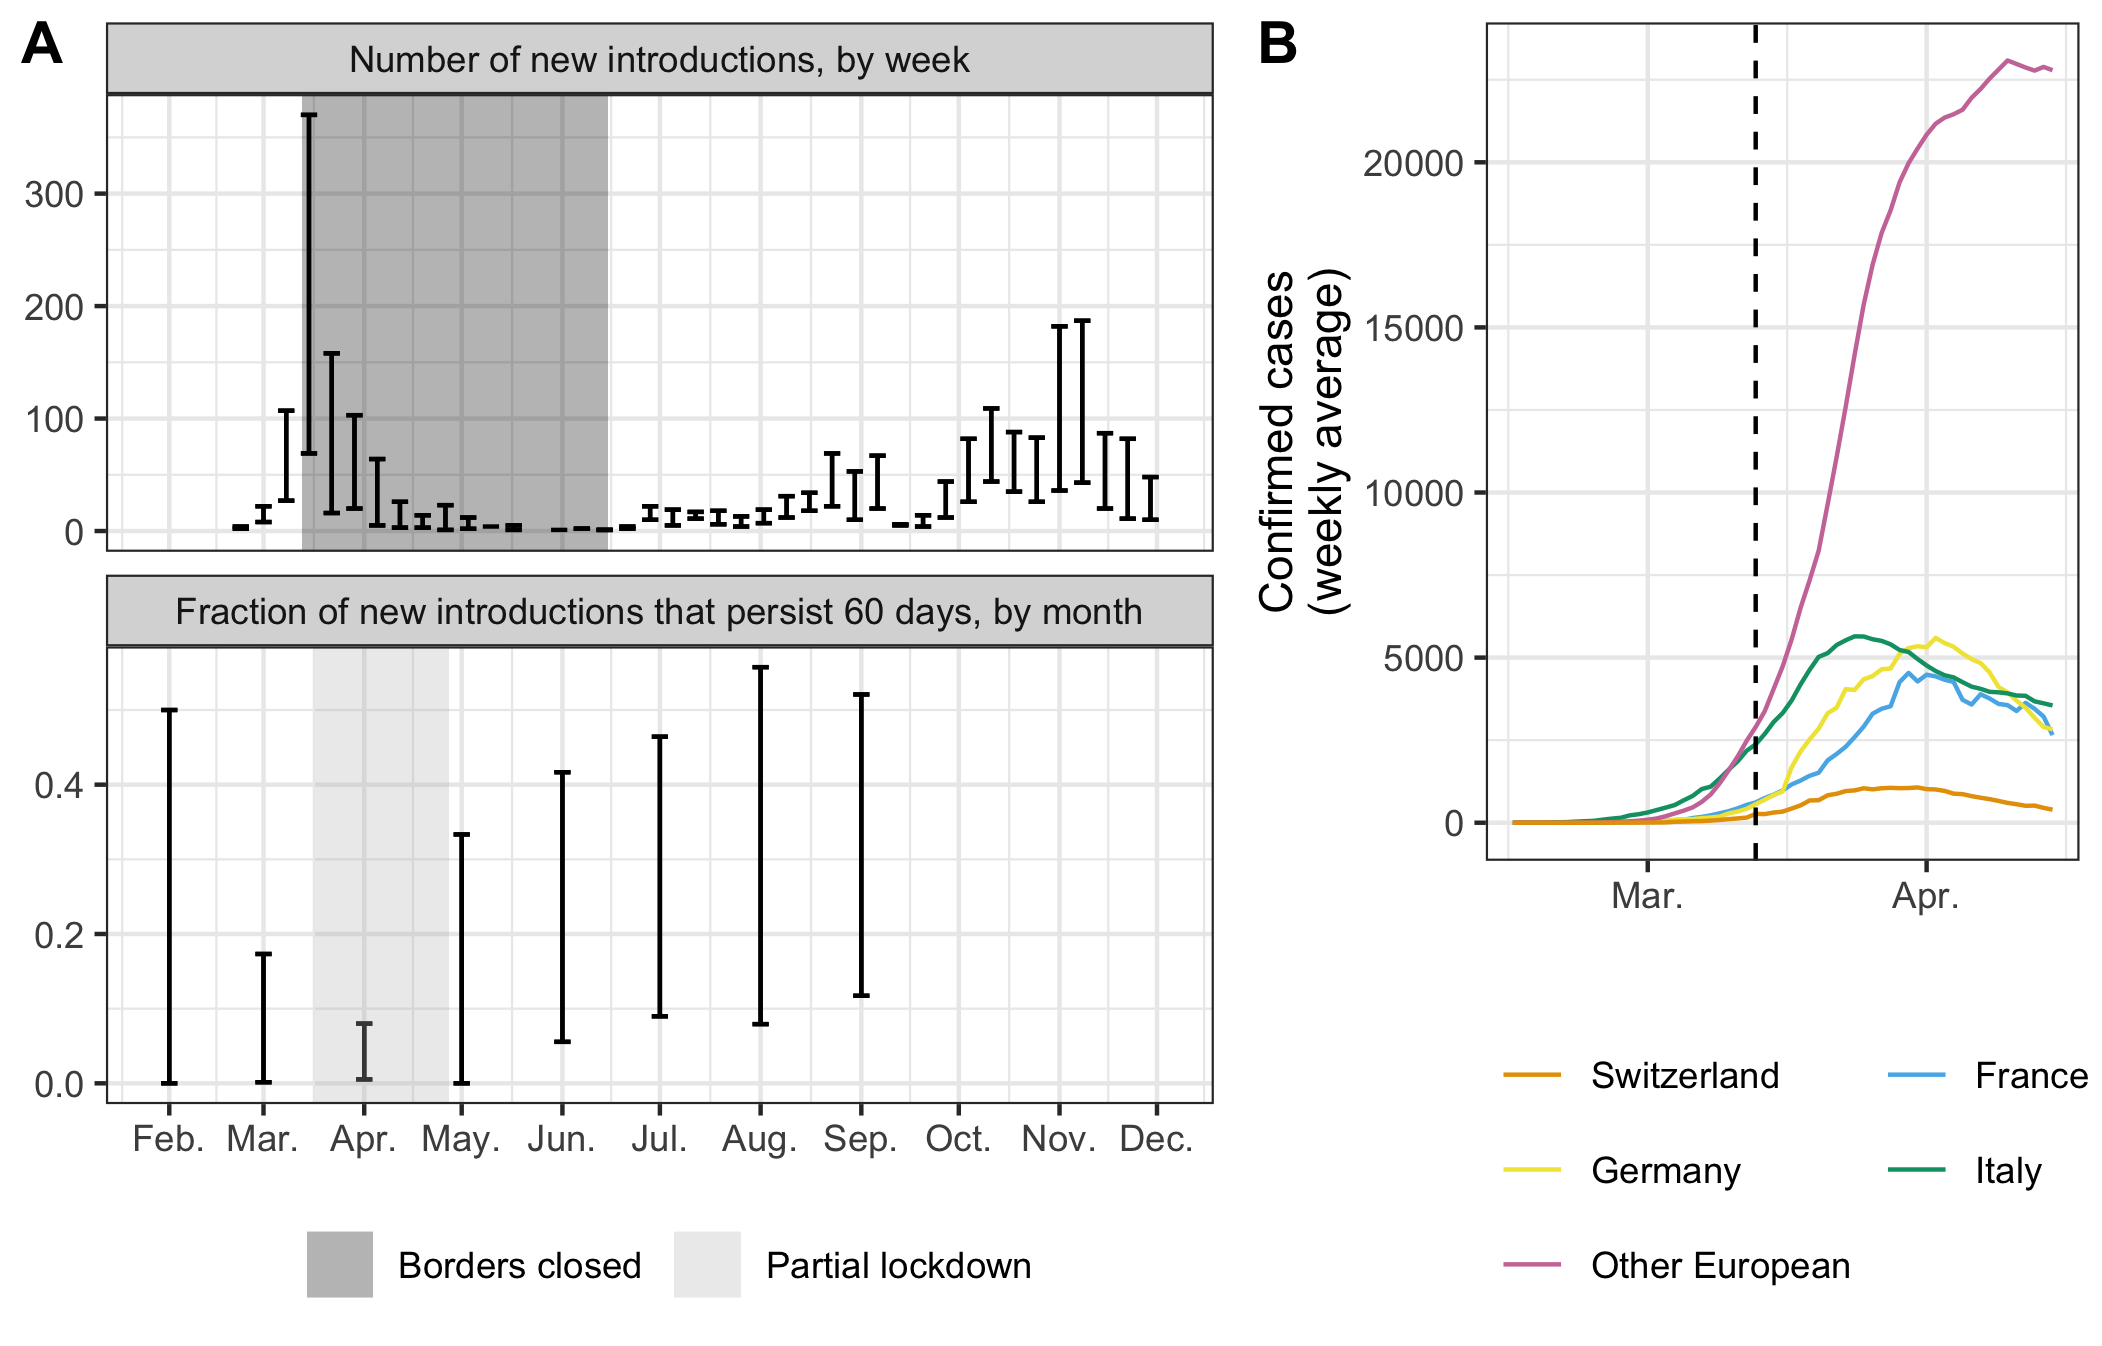
\includegraphics[width=0.75\linewidth]{figures/introductions_and_persistence.png}
\caption{A. Introductions into Switzerland and their persistence by the week (top) or month (bottom) they were first sampled. Persistence is defined by $\geq$ 60 days between the first sample and the latest sample. The error bars span two point estimates generated assuming either few or many introductions. The shaded rectangles highlight when the Swiss border closure (13. Mar. - 15. Jun.) and partial lockdown (17. Mar. - 27. Apr.) happened. Noteworthy, no estimates of the fraction of 60 days-persisting introductions could be made for new introductions occurring after 1st October, since our study only took into account sequences obtained until 1st December to avoid bias due to vaccine and to the alpha variant. B. For comparison, weekly average incidence by European country/region around the time of the Swiss border closures on 13. Mar. 2020 (dashed line). Case data here comes from the ECDC \cite{ECDC}.}
\label{fig:chain-longevity}
\end{figure}

\subsection{Genome data capture summer 2020 ``slowdown'' transmission dynamics}

Next, we investigated epidemic control once SARS-CoV-2 variants were introduced in Switzerland. Here, we quantified time-varying transmission dynamics in Switzerland in a Bayesian phylodynamic framework. We used a birth-death model with serial sampling, as originally described by \cite{stadler_2010_bds}. We conditioned the model on the introductions identified from our phylogenetic analysis. In a nutshell, our model assumes that once lineages are introduced, they are transmitted between hosts according to a shared time-varying transmission rate, die out upon recovery/death of the host according to a constant becoming-uninfectious rate, and yield genome samples with a time-varying sampling probability. We assume individuals who test positive adhere to the self-isolation regulations, so lineages die out when they are sampled. Under this parameterization, the effective reproductive number in Switzerland is a function of the transmission rate, becoming-uninfectious rate, and sampling probability.

We extended this methodology by adding a transmission rate ``damping'' factor to the implementation as shown in Figure \ref{fig:phylo-methods}. The implementation of this new method is available at TODO. The method aims to test whether contact tracing efforts in Switzerland slowed transmission once introductions were detected. We reasoned test-trace-isolate could slow transmission only shortly after the first case tests positive but not beforehand. We include this concept in our model by allowing the transmission rate to decrease by a multiplicative factor 2 days after each introduction is first sampled. The 2-day delay aims to account for the time between an individual giving a sample and having their contacts notified. This estimates is based on the time to RT-PCR results, which was generally lower than 24 hours in most Swiss laboratories, plus a small delay for contact tracers to reach the contacts \cite{Marquis2021}. Finally, we allowed the damping factor to vary between spring, summer, and fall in Switzerland - periods characterized by very different case loads and testing regimes (Figure \ref{fig:scale-factor}a). We used a spike-and-slab prior on this factor to include the possibility of no transmission slowdown. 

\begin{figure}[h!]
\centering
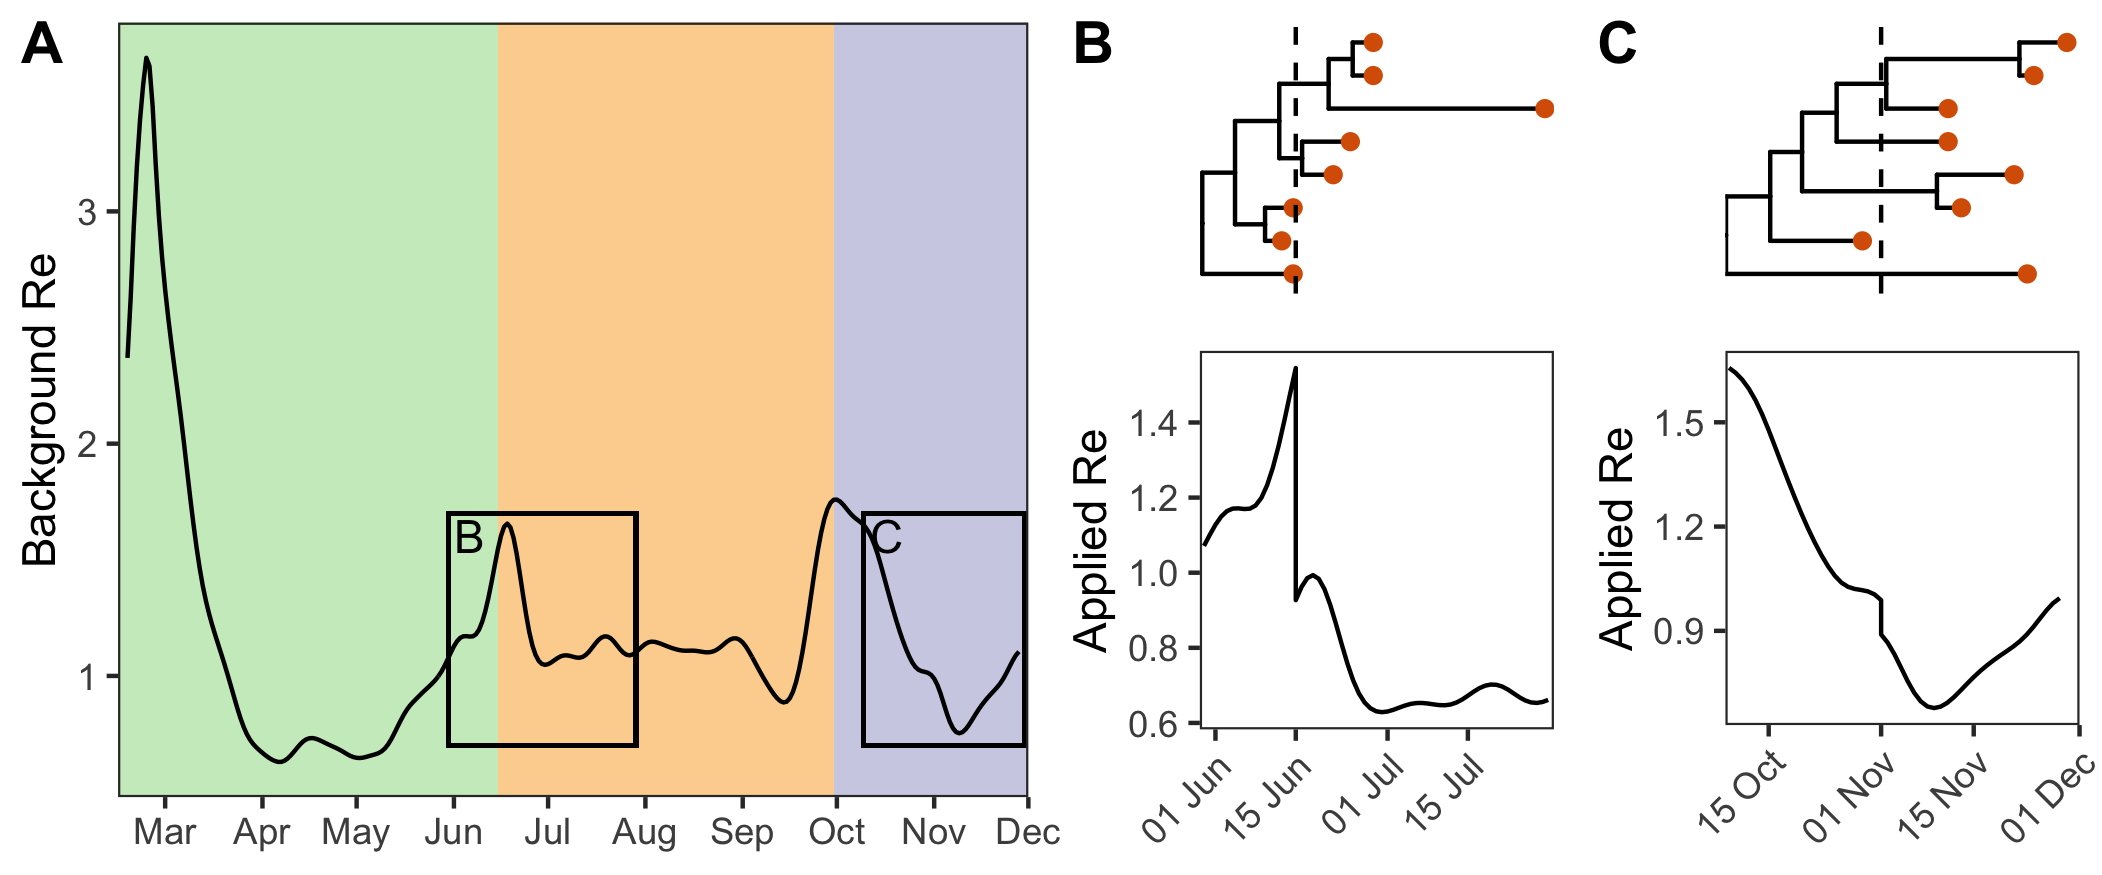
\includegraphics[width=0.75\linewidth]{figures/phylodynamic_method_example.png}
\caption{Illustration of how transmission rate damping is modelled. (A) shows a background time-varying reproductive number Re before any damping. In each of the coloured areas (Green = Spring, orange = Summer, and purple = Fall), a different transmission rate dampening factor is assumed. The black boxes in (A) highlight the spread of two example introductions (B) and (C). The genome data sampled from these introductions are shown as red dots in (B) and (C). The appropriate damping factor on Re is applied to each introduction 2 days after the first genome sample (dashed line). More concretely, in each step of the MCMC (Markov chain Monte Carlo) analysis, the background Re (A), the three dampening factors, and the two phylogenies (B and C) are sampled. The likelihood of the sampled genome data is calculated given the ``applied'' effective reproductive number specific to each introduction (B \& C, bottom).}  
\label{fig:phylo-methods}
\end{figure}

Across several model configurations (see supplemental text) and our two polytomy assumptions, we estimate effective reproductive number values through time that roughly capture the same trends as estimates based on confirmed case counts (Figure \ref{fig:ReSampProbResults}). On the other hand, sampling probability estimates in fall 2020 are strongly dependent on the prior (Figure \ref{fig:ReSampProbResults}), which we discuss more in the supplemental text.

Based on our main model configuration, we estimate a \summermaxdampingpercentmedianCHEnosampUB\ to \summermindampingpercentmedianCHEnosampUB\% slowdown in transmission after introductions are first sampled during summer 2020. In comparison, we estimate no or very little slowdown in relation to first sampling during fall 2020 (Figure \ref{fig:scale-factor}). These results are qualitatively robust to conditioning on few or many introductions and imposing a strong prior bound on the sampling proportion (Figure \ref{fig:DampingFactorResults}). In contrast, estimates in spring 2020 are inconsistent. This could be because low genomic diversity in SARS-CoV-2 during this period causes high phylogenetic uncertainty. In summary, we report an evident ``slowdown'' dynamic in SARS-CoV-2 transmission in Switzerland in Summer 2020 where transmission slows when the first genome sample analyzed is collected.

\begin{figure}[h!]
\centering
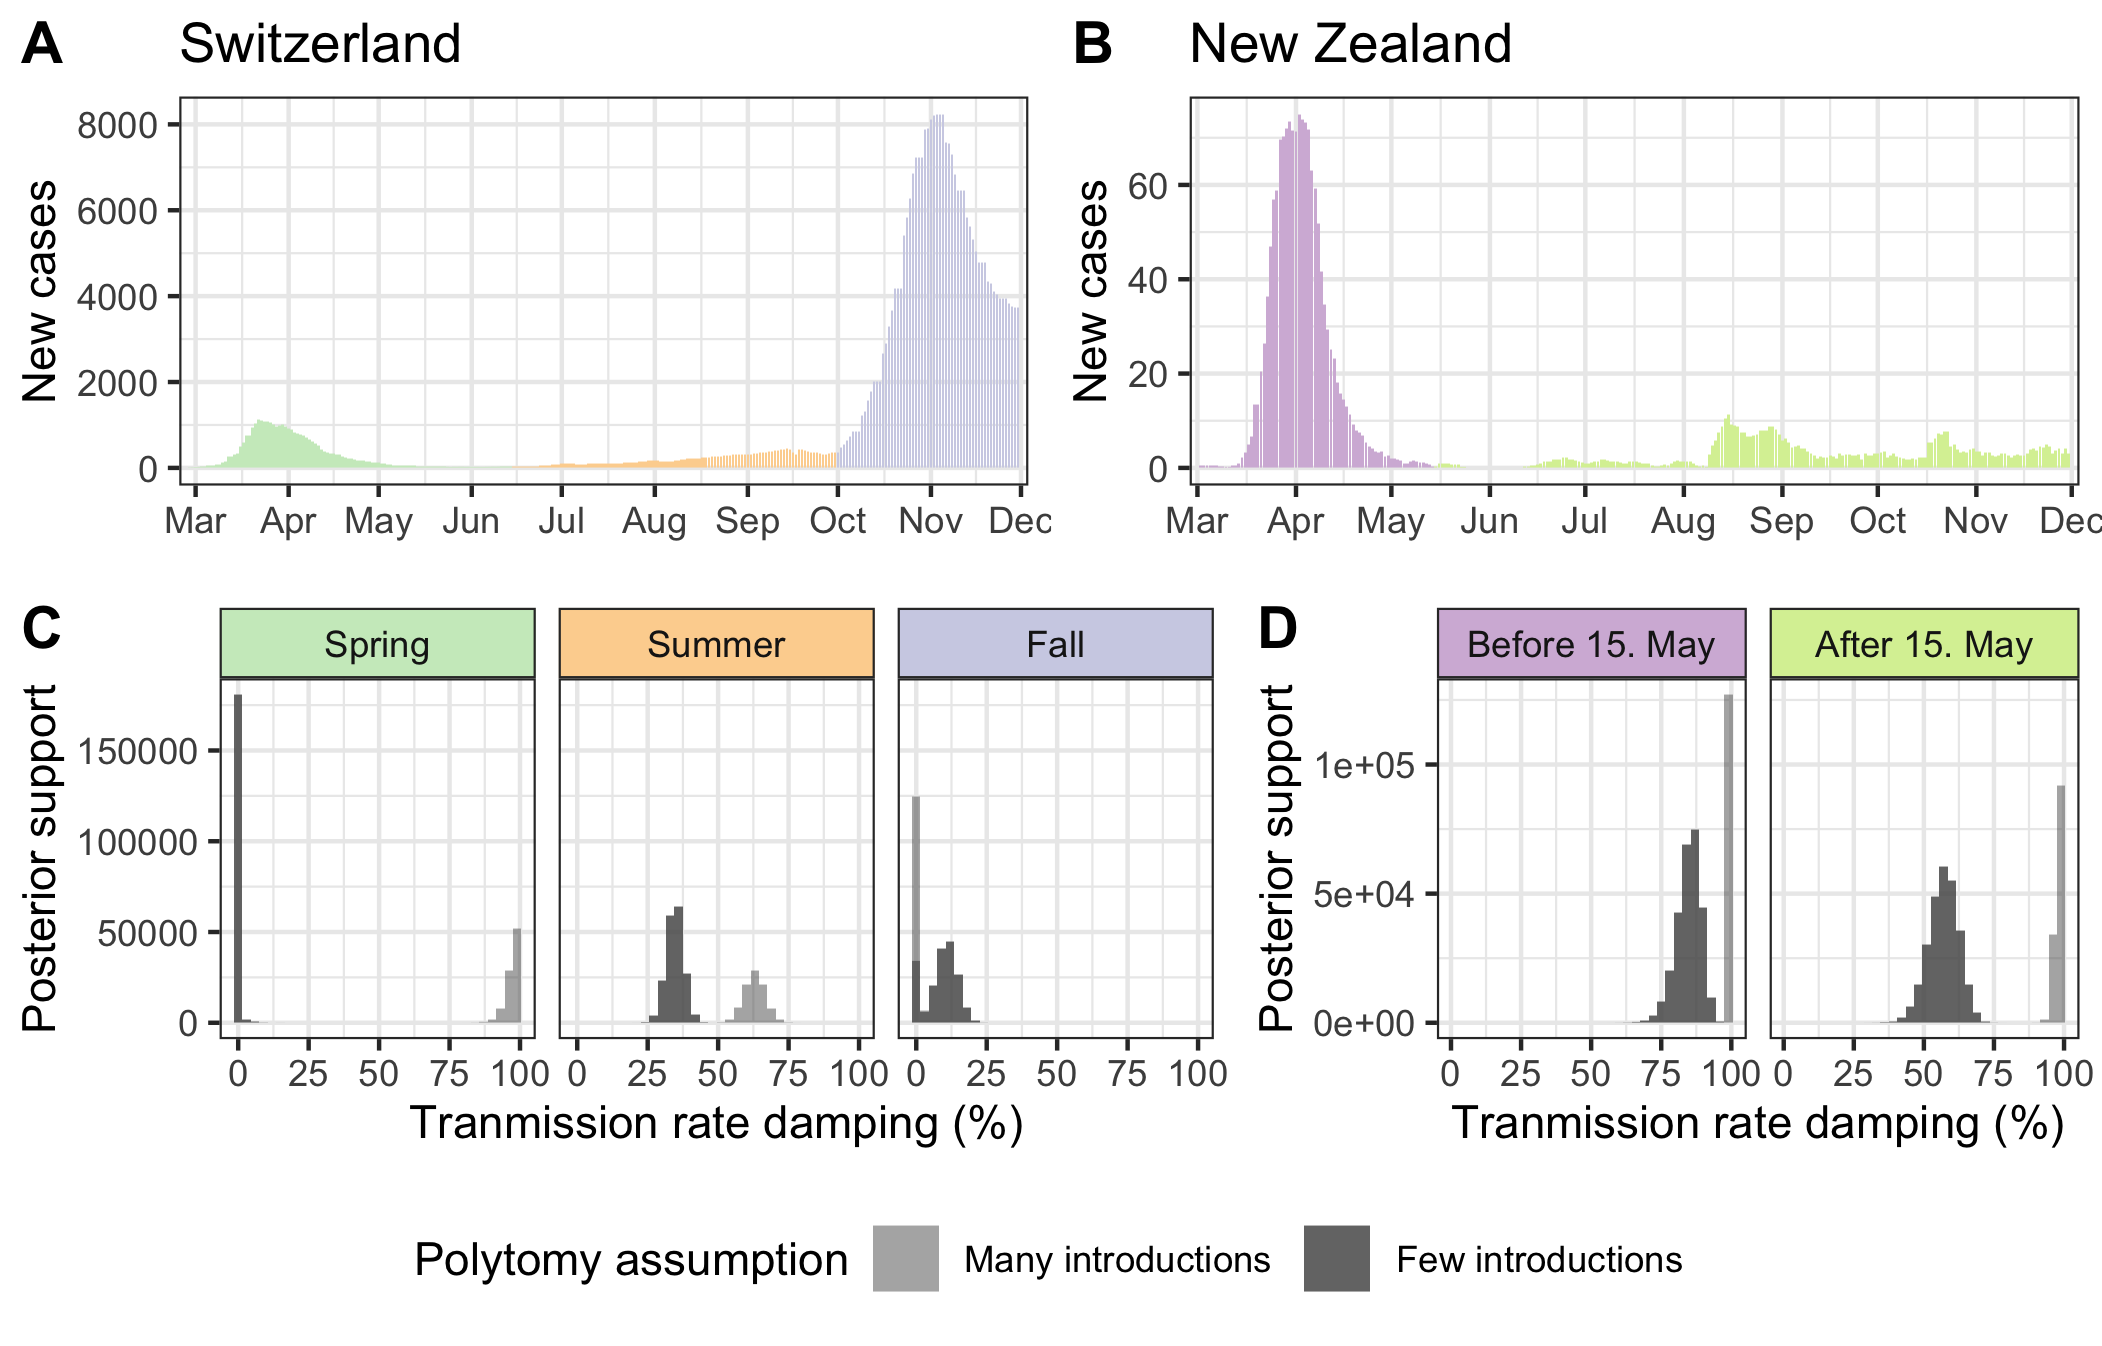
\includegraphics[width=0.75\linewidth]{figures/contact_tracing_factors_no_sampUB_compared_to_cases.png}
\caption{Epidemic trajectories in (A) Switzerland and (B) New Zealand during 2020 shown as a 7-day rolling average of daily new confirmed cases \cite{Appel}. (C) and (D) show estimates for if and how much transmission rates were dampened after introductions were sampled during different time periods in (C) Switzerland and (D) New Zealand. The inference was done twice, once conditioning on introductions identified assuming many introductions (light grey) and once assuming few introductions (dark grey). Thus, the difference between estimates in light and dark grey are due to phylogenetic uncertainty.}  
\label{fig:scale-factor}
\end{figure}

\subsection{Comparison to the New Zealand epidemic}
While Switzerland is centrally located in Europe and well-connected to other countries, especially those in the (normally) barrier-free Schengen travel zone, New Zealand is a relatively isolated island nation. Additionally, New Zealand aimed to eradicate SARS-CoV-2 throughout 2020 using strong measures, such as keeping its borders closed \cite{ZL-covid-policies}, while Switzerland re-opened to Europe in early Summer 2020. We compared our estimates for the transmission damping factor between Switzerland in spring, summer, and fall 2020 with New Zealand before and after an epidemic breakpoint in mid-May when local transmission was briefly eradicated \cite{Geoghegan2020}. From this point until early August, all cases in New Zealand were linked to managed quarantine facilities at the border. Then, a new community outbreak was identified on 11 August \cite{Geoghegan2021-nzl-outbreak}. Case numbers were subsequently held at lower levels through Dec. 2020 (Figure \ref{fig:DampingFactorResults}B). Based on the available genome data from New Zealand, which includes samples linked to managed quarantine facilities and from the community, we estimated damping factors in New Zealand before and after 15. May to be comparable or stronger than in Switzerland during Summer and Fall 2020 (Figure \ref{fig:scale-factor}).

\section{Discussion}
% Re-state the goal and the main results
We aimed to assess genomic evidence for the impact of major public health measures on SARS-CoV-2 transmission in Switzerland. We estimate that the Swiss border closure on 16. Mar. 2020 caused new introductions of SARS-CoV-2 to peak before cases in Switzerland's neighboring countries and the rest of Europe. Without this intervention, we  expect new introductions would have continued rising with cases in neighboring regions until early to mid-April. The border closure was mostly lifted again on 15. Jun 2020. Correspondingly, we estimated week-on-week increases in the number of new introductions throughout summer 2020. Next, we estimated that introductions spreading during the spring 2020 lockdown were more likely to be driven to extinction compared to later introductions. Only 0.5 - 8\% of April introductions persisted more than 60 days, compared to 12 - 52\% of Septemper introductions. Finally, we quantified a summertime ``slowdown'' dynamic in which introductions initially spread faster, then slowed between \summermaxdampingpercentmedianCHEnosampUB\ and \summermindampingpercentmedianCHEnosampUB \%. Together, these results show the efficacy of border closure and lockdown, and potentially, quantify the efficacy of test-trace-isolate implementation, in Switzerland.

% Contextualize the results: caveats
It is important to interpret these results in light of the data and methods used, and their limitations. Most obviously, estimates on the number, timing, and duration of introductions are very uncertain due to incomplete sampling and phylogenetic uncertainty. Others have struggled with the same challenges \cite{Morel2021} and we support their conclusion: one should consider estimates generated across a range of plausible phylogenies, as estimates based on any one phylogeny may be misleading. In our analysis, we present estimate ranges based on two extreme resolutions of polytomies. This is less computationally intensive, but more conservative, compared to generating a larger set of plausible phylogenies as in Bayesian analyses and as \cite{Morel2021} suggested for maximum-likelihood analyses.

Further, genomic data are observational data and subject to potential sampling biases. Available sequences may not represent the overall infected population due to time-varying testing regimes, geographic or demographic sampling biases, and demographic skew in disease severity. In particular, we expect severe cases, contacts of positive cases, and populations with better access to testing or better sequencing coverage are sampled more. To avoid some of these biases, we used our own sequences and other sequences collected across Switzerland and down-sampled the regions and time periods where sequences were over-represented compared to case numbers. Thus, we argue that our final data set is representative of trends in transmission dynamics through time. We caution against interpreting the absolute numbers of introductions identified and the persistence of any specific introduction. Finally, we expect changes through time to be primarily due to non-pharmaceutical interventions or seasonal effects because our sampling period is prior to the identification of more transmissible variants of concern and prior to vaccines being available. 

% Contextualize the results: interpretations
Despite these limitations, a major benefit of using whole-genome sequencing data is that we can link related cases. This allows us to identify independent introductions and to investigate transmission dynamics within introductions. Here, we hypothesized that test-trace-isolate measures should slow transmission within introductions once they are sampled. Without genomic data to differentiate cases into independent introductions and chains of transmission, this would only be possible if detailed contact tracing data were to become available. Recently, \cite{Fetzer2021} exploited an accidental, partial breakdown of English contact tracing to show that English contact tracing in early fall 2020 reduced transmissions in the 6 weeks following a positive case by 63\%. Here we use a different data source - whole-genome sequences - and, uniquely, track transmission dynamics within introductions. The measured efficacy of English contact tracing in early fall 2020 is within the range of our estimates for a transmission slowdown in Switzerland in summer 2020.

Although we hypothesize that a transmission ``slowdown'' should reflect test-trace-isolate measures, there could be other factors at play. First, extensive backwards and forwards contact tracing would have been necessary to simultaneously slow all sister lineages of the lineage first sampled, as we assume. Informal backwards contact tracing by individuals themselves may have helped, but likely not to the extent we assume. Instead, it is possible other factors helped the slowdown. For one, returning travellers have been implicated in transmitting more than non-travellers \cite{Hodcroft2021} during times of lifted restrictions as in summer 2020. Thus, a passive transmission slowdown might happen when the virus moves into the non-traveller population. However, we would expect travellers in fall to have similar contact networks as those in summer. Instead, transmission damping is only evident in Switzerland in summer 2020 when case counts were low. This could be because manual contact tracing (as in Switzerland) likely functions better when overall case loads are low. When case numbers were high in fall, Swiss contact tracing was reported to struggle \cite{SWI-contact-tracing-failing}. We also quantified a similar slowdown effect in New Zealand during two different time periods, indicating this effect is not unique to Switzerland during summer. \cite{Mendes2021} used genome sequence data to show that New Zealand contact tracing was highly effective in identifying SARS-CoV-2 infection clusters. Further, New Zealand is known for intense contact tracing efforts and quarantine for travellers \cite{ZL-covid-policies}. A second alternate explanation for the slowdown dynamic might be that contacts of positive cases are tested more intensely. For instance, close contacts are encouraged to get tested, yielding an apparent ``burst'' of samples around the first detected case. If so, we can still interpret the slowdown dynamic as evidence that test-trace-isolate implementation was working, but it is difficult to determine precisely how much transmission actually slowed.

% Argue for importance
Our findings highlight the effect of major public health measures on the Swiss epidemic. Our analysis suggests that strict public health measures like the partial border closure and lockdown in spring 2020 helped prevent and contain new introductions. However, these measures are naturally unsustainable. We estimate that when case counts are maintained at a low level, as in summer 2020 in Switzerland and in New Zealand, new introductions initially spread more quickly, but then slowed down. Estimates from fall 2020 in Switzerland show that no such slowdown occurred when case counts were high. We speculate this is due to test-trace-isolate resources being overwhelmed. In conclusion, our results argue for the benefits of contact tracing efforts, thoughtful quarantine policies, and the benefits of maintaining case counts at a low level to enable outbreak control while vaccines are distributed and treatment options continue to improve.

\acknow{This work was supported by the Swiss National Science Foundation (SNSF) through grant number 31CA30\_196267 (to TS). We gratefully acknowledge the authors from the originating laboratories responsible for obtaining the specimens and the submitting laboratories where genetic sequence data were generated and shared via the GISAID Initiative, on which this research is based. A full acknowledgements table of these groups, including the identifiers for all GISAID data used in this study, is available on the project GitHub repository at TODO. We also thank Jana Huisman for valuable discussions on the manuscript.}

\showacknow{} % Display the acknowledgments section

% Bibliography
\printbibliography

\end{document}
